\documentclass[mathserif, aspectratio=169]{beamer}
%
%%%%%%%%%%%%%%%%%%%%%%%%%%%%%%%%%%%%%%%%%%%%%%%%%%%%%%%%%%%%%%%%%%%%%%%%
% need to split the includes to make spell checking work.
\usepackage{arev, arevmath}
\usepackage[scaled]{cabin}
\usepackage[T1]{fontenc}
\usepackage[super]{nth}
\usepackage{pifont}
\usepackage{wasysym}
\usepackage{tabularx}
\usepackage{array}
\usepackage{booktabs}
\usepackage{boldline}
\usepackage{colortbl}
%\usepackage{amsmath}
\usepackage{bm}
\usepackage{tcolorbox}
\usepackage{adjustbox}
\usepackage{minibox}
\usepackage{makecell}
\usepackage{adjustbox}
\usepackage{textcomp}
\usepackage[absolute,overlay]{textpos}
\setlength{\TPHorizModule}{1mm}%
\setlength{\TPVertModule}{1mm}%
\tcbuselibrary{skins}

\makeatletter
\newcommand{\antsize}{\@setfontsize{\antsize}{4pt}{4pt}}
\makeatother
\newcommand{\at}{\makeatletter @\makeatother}

\newcommand{\cmark}{\ding{51}}%
\newcommand{\bottomline}[1]{\vskip0pt plus 1fill{\alert{#1}\phantom{g}\vskip 1.0mm}}

\newcommand{\Quote}[2]{%
	\begin{center} 
		\begin{minipage}{0.7\textwidth} 
			\hrule
			\vskip 3mm
			\emph{{\color{ICTPblue} ``#1''}
			
			~~~~ {\color{ICTPorange} --- #2}}
			\vskip 3mm
			\hrule
			\vskip 2mm
		\end{minipage}
	\end{center}}


\mode<presentation>%
{
	\usetheme{default}
	%\usetheme[width=2.5cm]{PaloAlto}
	\usecolortheme{dove}
	\useoutertheme{infolines}
	% oder auch nicht

	% ICTP Colors
	\definecolor{ICTPblue}{RGB}{37,86,162} % 0x255682
	\definecolor{ICTPorange}{RGB}{255,130,0} % 0xff8200
	\definecolor{ICTPgreen}{RGB}{0,100,0}
	\definecolor{ICTPdark}{RGB}{80,80,80} % 0x505050
	\definecolor{ICTPlight}{RGB}{120,120,120}
	\definecolor{ICTPbrown}{RGB}{178,91,0}

	\definecolor{codebg}{rgb}{0.95,0.95,0.95}

	% Color theme
	\setbeamercolor{alerted text}{fg=ICTPorange}
	\setbeamercolor{frametitle}{fg=ICTPblue}
	\setbeamercolor{title}{fg=ICTPblue}
	\setbeamercolor{subtitle}{fg=ICTPorange}
	\setbeamercolor{normal text}{fg=ICTPdark}
	\setbeamercolor{author in foot}{fg=ICTPblue}
	\setbeamercolor{item}{fg=ICTPblue}
	\setbeamercolor{footline}{fg=ICTPblue}
	%\setbeamercolor{item projected}{bg=ICTPorange}
	%\setbeamercolor{item projected}{fg=white}

	\setbeamertemplate{headline}
	{}
	\setbeamertemplate{frametitle}
	{
		%\textbf{{\insertframetitle\phantom{g}}}\\
		%\textbf{\insertframetitle\phantom{g}}\\
		\textbf{\underline{\insertframetitle\phantom{g}}}\\
		%\textbf{\underline{\insertframetitle}}\\
		\vskip 1.0mm
		%{\color{UOLgold}\hrule height 2pt}
		%\par
	}
	\addtobeamertemplate{frametitle}{}{\vspace{-1em}}
	\setbeamertemplate{footline}{
		{%
			\textbf{ \hskip 3.0mm\insertshorttitle\phantom{.}---\phantom{.}\insertshortinstitute\hfill\insertframenumber\,/\,\inserttotalframenumber\hskip 3.0mm} 
		}
	}

	\setbeamertemplate{navigation symbols}{}%remove navigation symbols
	\setbeamertemplate{itemize items}[circle]
	\setbeamertemplate{enumerate items}[fg=ICTPblue]
	\setbeamercolor{itemize items}{fg=ICTPblue}
	\setbeamercolor{sidebar}{bg=ICTPblue}
	\setbeamercolor{title in sidebar}{fg=ICTPorange}
	\setbeamercolor{author in sidebar}{fg=ICTPorange}
	\setbeamercolor{section in sidebar}{fg=ICTPorange}
}

%\input{tikz/common-styles}

\usepackage{graphicx}
\usepackage[latin1]{inputenc}

\graphicspath{{../figs/}{../figs/common/}{../figs/islr/}}

\title[Statistical Learning] % (optional, nur bei langen Titeln n�tig)
{\textbf{Introduction to Statistical Learning\\ {\it with applications in Python}}\\%
		\href{www.statlearning.com}%
		{\tiny\it Based on ``Introduction to Statistical Learning, with applications in R'' by Gareth James, Daniela Witten, Trevor Hastie, Robert Tibishirani}\vspace{2em}}
		\vspace{-2.5cm}{}


		\author{\href{mailto:?to=Kurt Rinnert <kurt.rinnert@cern.ch>&subject=PWF Statistical Learning}{Kurt Rinnert}}

\institute[{\href{https://www.ictp.it/physics-without-frontiers.aspx}{Physics Without Frontiers} --- \href{https://www.ictp.it/}{ICTP}}] % (optional)
{\color{ICTPblue}\bfseries \href{https://www.ictp.it/physics-without-frontiers.aspx}{Physics Without Frontiers}\\\vspace{1mm}%
\href{https://www.ictp.it/}{
\includegraphics[width=0.20\textwidth]{common/ICTP-logo-full-trans.png}}\\%
\href{https://www.liverpool.ac.uk/physics/}{
\includegraphics[width=0.2\textwidth]{common/uol_logo.png}}}

\date{}

\titlegraphic{
	\texorpdfstring{\vspace{-2.8cm}}{}
	 \begin{minipage}[b][1.3cm][b]{0.26\textwidth}\color{ICTPlight}\antsize
		Copyright \textcopyright~2019\\
		\href{mailto:?to=Kurt Rinnert <kurt.rinnert@cern.ch>&subject=PWF Statistical Learning}{Kurt Rinnert <kurt.rinnert{\tt @}cern.ch>},
		\href{mailto:?to=Kate Shaw <kshaw@ictp.it>&subject=PWF Statistical Learning}{Kate Shaw <kshaw{\tt @}ictp.it>}\\
		Copying and distribution of this file, with or without modification,
		are permitted in any medium without royalty provided the copyright
		notice and this notice are preserved.  This file is offered as-is,
		without any warranty.


		Some of the figures in this presentation are taken from ``An Introduction to
		Statistical Learning, with applications in R''  (Springer, 2013) with
		permission from the authors: G. James, D. Witten,  T. Hastie and R. Tibshirani 
	 \end{minipage}\hspace{10cm}
}


\addtocounter{framenumber}{-1}

% nicer table row separation
\renewcommand{\arraystretch}{1.2}

% color boxes
\newcommand{\tabboxset}{\tcbset{enhanced, nobeforeafter, boxrule=0pt, boxsep=0pt, colback=codebg, colframe=codebg, coltext=ICTPdark, rounded corners, arc=4pt, fonttitle={\bfseries\tiny}}}
\newcommand{\codeboxset}{\tcbset{enhanced, nobeforeafter, boxrule=0pt, boxsep=0pt, colback=codebg, colframe=codebg, coltext=ICTPdark, rounded corners, arc=4pt, fonttitle={\bfseries\tiny}}}

\newcommand{\orange}{\color{ICTPorange}}
\newcommand{\blue}{\color{ICTPblue}}
\newcommand{\dark}{\color{ICTPdark}}
\newcommand{\R}{\mathbb{R}}
\newcommand{\dat}[1]{{\footnotesize\tt\orange #1}}
\newcommand{\e}[1]{\emph{#1}}
\newcommand{\bh}{\hat{\beta}}
\newcommand{\h}{\hat}

\makeatletter
\newcommand{\includegraphicsdpi}[3]{%
	\pdfimageresolution=#1%
	\includegraphics[#2]{#3}%
	\pdfimageresolution=72%
}

\newenvironment{blurb}%
	{\begin{center}\begin{minipage}{0.6\textwidth}\footnotesize}
	{\end{minipage}\end{center}}

\newenvironment{cpage}%
	{\begin{center}\begin{minipage}{0.75\textwidth}}
	{\end{minipage}\end{center}}

\newenvironment{popblock}[2]%
	{\begin{center}\begin{minipage}{#1}\footnotesize
		\begin{tcolorbox}[colframe=codebg, colback=white, colupper=ICTPdark, title={\normalsize\bfseries\blue #2}]}
	{\end{tcolorbox}\end{minipage}\end{center}}
\makeatother

\subtitle{\bfseries%
  {Linear Regression, Part 2}\\%
  {\tiny\it multiple linear regression, hypothesis testing, important variables, fit quality, predictions}\\%
}
\begin{document}
\frame[plain]{
	\vskip 1.0mm
	\titlepage
	\vskip 1.0mm
}


\begin{frame}{Abstract}

	\begin{blurb}
		Linear models are an important topic in statistical learning.  

		The true relationships between predictors and responses are rarely linear.
		But linear models often provide reasonable approximation. They provide
		high interpretability and have low variance, mitigating the risk of over-fitting.
		Linear models can be extended to include (some) non-linear relationships. 

		Linear models also provide an excellent baseline to compare other models against: if 
		our sophisticated model does not do much better than a linear model we might consider
		trading some bias for lower variance.
	\end{blurb}
\end{frame}

\begin{frame}{Overview}
	\begin{itemize}
		\item Linear models with multiple predictors.
		\item Hypothesis testing, the $F$-statistic.
		\item Choosing important variables.
		\item Assessing the fit \& prediction quality.
	\end{itemize}
	\bottomline{This will require some mathematics.}
\end{frame}

\begin{frame}{The Scenario}
	\begin{itemize}
		\item We look at the \dat{Advertising} data set again.
		\item Previously, we only used the \dat{TV} predictor to predict \dat{sales}.
		\item The data set provides two more predictors, \dat{radio} and \dat{newspaper}.
		\item We are now interested in using all available information in the data set.
		\item We can think of two ways of doing that:
			\begin{cpage}
				\begin{enumerate}
					\item Perform simple linear regression on the predictors separately.
					\item Somehow combine all predictors.
				\end{enumerate}
			\end{cpage}
	\end{itemize}
	\bottomline{As you might guess, option two is more interesting, but let's look at option one first.}
\end{frame}

\begin{frame}{Separate Simple Linear Regression}
	\begin{center}
		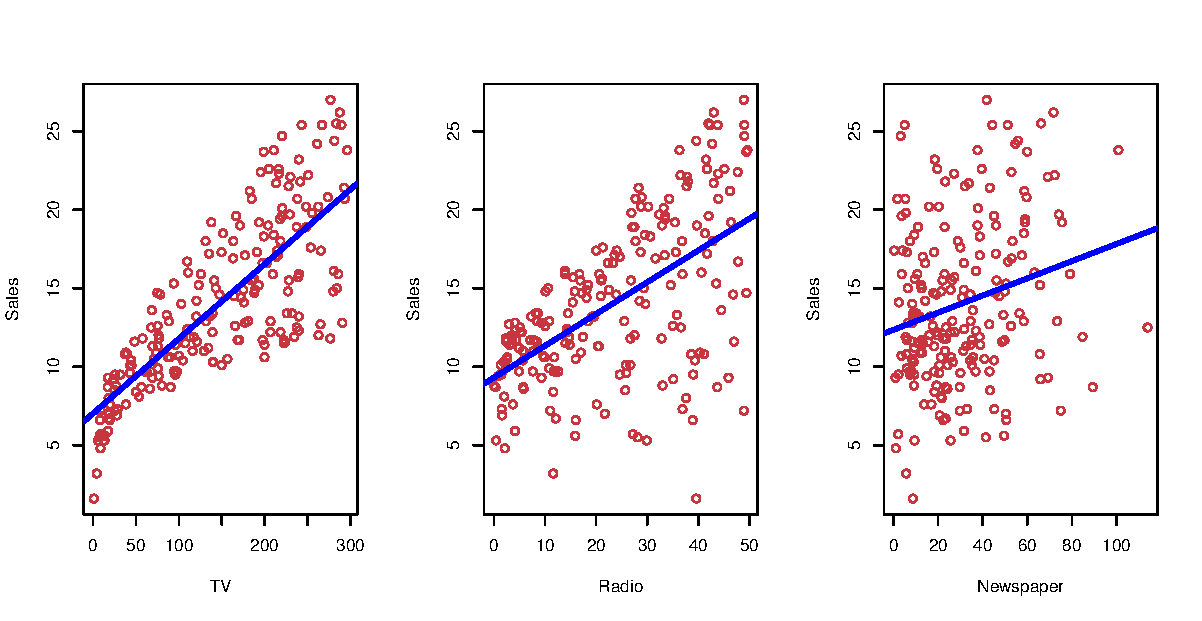
\includegraphics[width=0.7\textwidth]{2_1}
	\end{center}
	\bottomline{Separate simple linear regression looks promising on this data set.}
\end{frame}

\begin{frame}{Separate Simple Linear Regression}
	\begin{popblock}{0.7\textwidth}{Regression of \dat{sales} onto \dat{radio}}
		\begin{tabular}[h]{lrrrr}
			{} & {\blue Coefficient} & {\blue Std. Error} & {\blue $t$-statistic} & {\blue $p$-value} \\
			\dat{Intercept} & 9.312 & 0.563 & 16.54 & $< 0.0001$ \\
			\dat{radio} & 0.203 & 0.020 & 9.92 & $< 0.0001$ \\
		\end{tabular}
	\end{popblock}
	\begin{popblock}{0.7\textwidth}{Regression of \dat{sales} onto \dat{newspaper}}
		\begin{tabular}[h]{lrrrr}
			{} & {\blue Coefficient} & {\blue Std. Error} & {\blue $t$-statistic} & {\blue $p$-value} \\
			\dat{Intercept} & 12.351 & 0.621 & 19.88 & $< 0.0001$ \\
			\dat{newspaper} & 0.055 & 0.017 & 3.30 & $ 0.00115$ \\
		\end{tabular}
	\end{popblock}
	\bottomline{All the separate regressions look reasonable.}
\end{frame}

\begin{frame}{Separate Simple Linear Regression}
	\begin{itemize}
		\item This is not entirely satisfactory for several reasons.
		\item It is unclear how could predict a single value of \dat{sales} from
			the separate models.
		\item Each of the separate models ignores the other variables.
		\item This is problematic if there are correlations between the predictors.
	\end{itemize}
	\bottomline{A better approach is to use multiple predictors simultaneously.}
\end{frame}


\begin{frame}{Multiple Simple Linear Regression}
	\begin{itemize}
		\item \e{Multiple linear regression} uses multiple predictors.
		\item Each predictor has its own slope coefficient.
		\item For $p$ predictors the model takes the form
			\[ Y = \beta_0 + \beta_1 X_1 + \beta_2 X_2 + \dots + \beta_p X_p + \epsilon \]
			where the $\beta_j$ are interpreted as the average effect $X_j$ has on $Y$ while\\
			\e{holding all other predictors constant}.
		\item For example:
			\[ \text{\dat{sales}} = \beta_0
				+ \beta_1\times\text{\dat{TV}}
				+ \beta_2\times\text{\dat{radio}}
				+ \beta_3\times\text{\dat{newspaper}}
				+ \epsilon
			\]
	\end{itemize}
	\bottomline{Now we have one model using all the information.}
\end{frame}

\begin{frame}{Example: Two Predictors}
	\begin{center}
		\vspace{-5mm}
		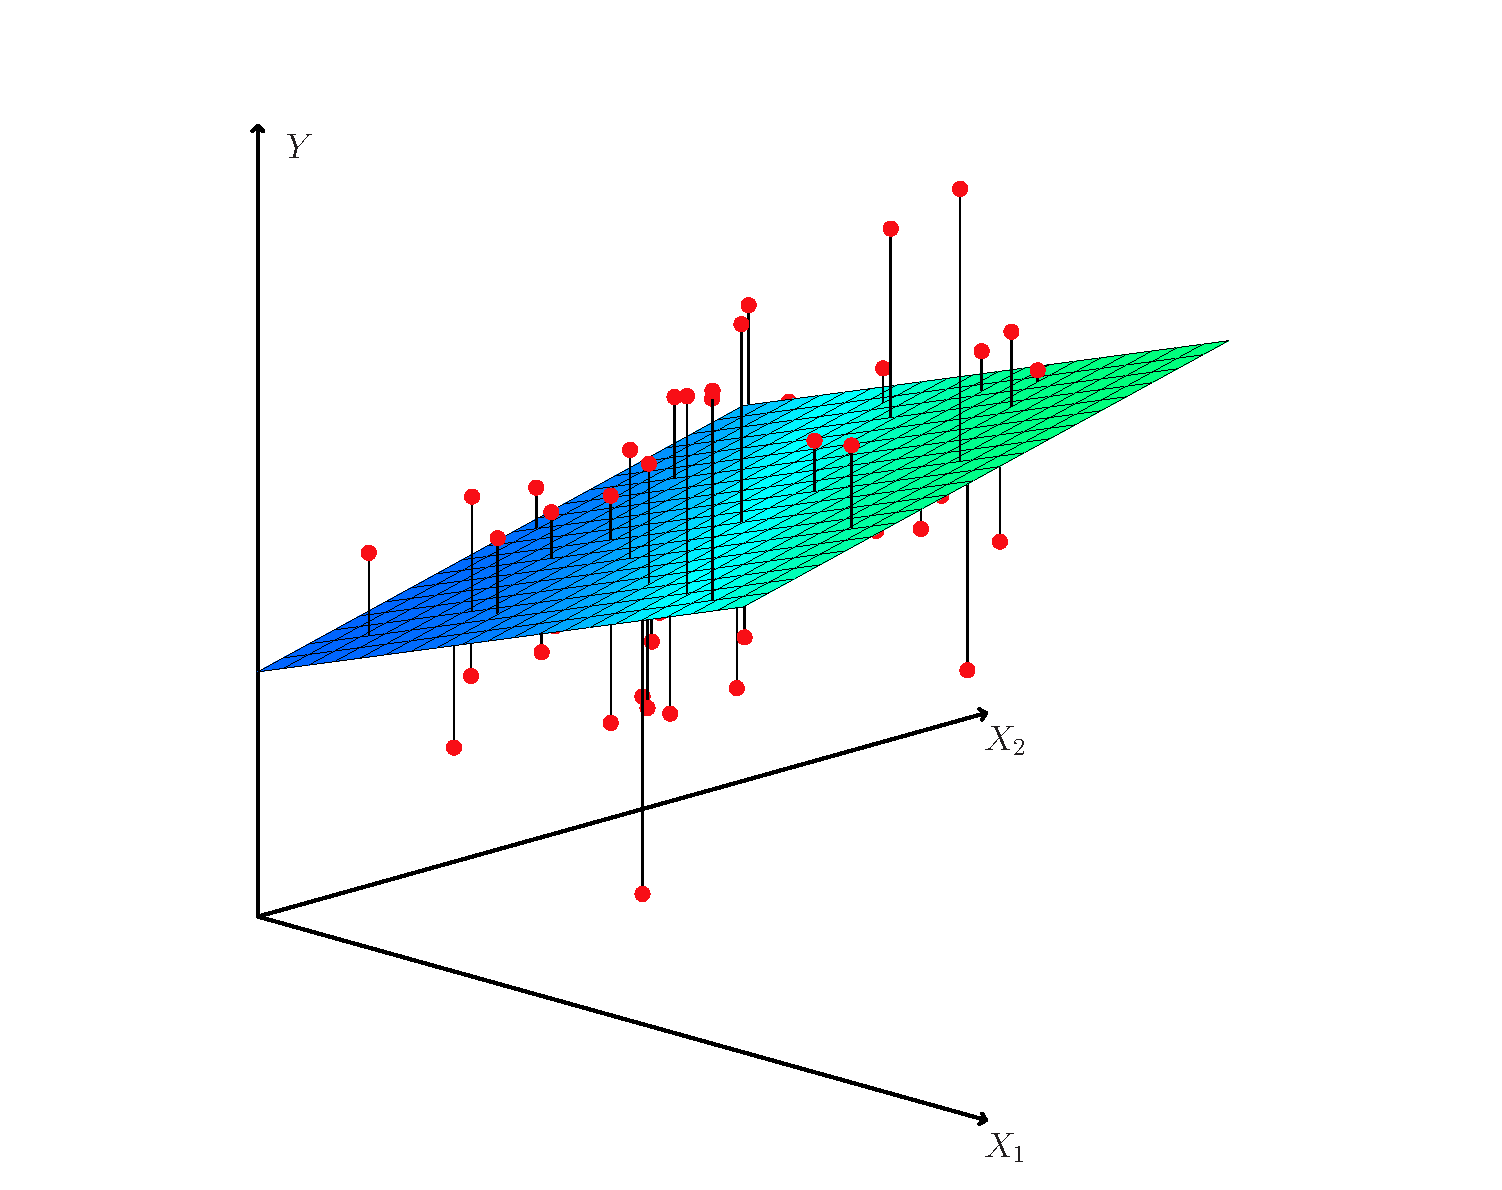
\includegraphics[width=0.5\textwidth]{3_4}

		\vspace{-8mm}
		\[ Y = \beta_0 + \beta_1 X_1 + \beta_2 X_2 + \epsilon \]
	\end{center}
	\bl{In general, the result is a \e{hyperplane}.}
\end{frame}

\begin{frame}{Estimating the Regression Coefficients}
	\begin{itemize}
		\item As in simple linear regression we want to make predictions using
			estimated parameters:
			\[ \h{y} = \bh_0 + \bh_1 x_1 + \bh_2 x_2 + \dots + \bh_p x_p \]
		\item We choose the coefficients $\bh_0, \bh_1, \bh_2, \dots, \bh_p$
			to minimise the sum of squared residuals:
			\begin{align*}
				\text{RSS} &= \sum_{i=1}^n (y_i - \hat{y}_i)^2 \\
				{} &= \sum_{i=1}^{n} (y_i - \bh_0 - \bh_1 x_1 - \bh_2 x_2 - \dots - \bh_p x_p)^2
			\end{align*}
	\end{itemize}
	\bl{Deriving the solution involves some matrix manipulations.}
\end{frame}

\begin{frame}{Estimating the Regression Coefficients}
	\begin{columns}[t]
		\begin{column}{0.5\textwidth}
			\begin{itemize}
				\item Recall the notation for the \e{feature matrix}:
					\begin{align*}
						\bm{X} &=
						\begin{pmatrix}
							x_{11} & x_{12} & \dots & x_{1{\orange p}} \\ 
							x_{21} & x_{22} & \dots & x_{2{\orange p}} \\ 
							\vdots & \vdots & \ddots & \vdots \\
							x_{{\blue n}1} & x_{{\blue n}2} & \dots & x_{{\blue n}{\orange p}} \\ 
						\end{pmatrix}\in \R^{{\blue n}\times{\orange p}}\\
					\end{align*}
			\end{itemize}
		\end{column}
		\begin{column}{0.5\textwidth}
			\begin{itemize}
				\item We define the vectors:
					\vspace{2mm}
					\begin{align*}
						\bm{\beta_0} &= (\beta_0, \beta_0, \dots, \beta_0)^T &\in \R^{\blue n} \\
						\beta &= (\beta_1, \beta_2, \dots, \beta_{\orange p})^T &\in \R^{\orange p}\\
						\bm{\epsilon} &= (\epsilon_1, \epsilon_2, \dots, \epsilon_{\blue n})^T &\in \R^{\blue n}\\
					\end{align*}
			\end{itemize}
		\end{column}
	\end{columns}
	\begin{itemize}
		\item With this and the convention for the response vector $\bm{y} \in \R^{\blue n}$ we can write
			the model as
			\[
				\bm{y} = \bm{\beta_0} + \bm{X}\beta + \bm{\epsilon}
			\]
	\end{itemize}
	\bl{These are $\bm{n}$ simultaneous equations describing the linear model.}
\end{frame}

\begin{frame}{Estimating the Regression Coefficients}
	\begin{columns}[t]
		\begin{column}{0.5\textwidth}
			\begin{itemize}
				\item We now redefine $\bm{X}$ to obtain the\\
					model's \e{design matrix}:
					\begin{align*}
						\bm{X} &=
						\begin{pmatrix}
							1 & x_{11} & x_{12} & \dots & x_{1{\orange p}} \\ 
							1 &x_{21} & x_{22} & \dots & x_{2{\orange p}} \\ 
							\vdots & \vdots & \vdots & \ddots & \vdots \\
							1 & x_{{\blue n}1} & x_{{\blue n}2} & \dots & x_{{\blue n}{\orange p}} \\ 
						\end{pmatrix} \in \R^{{\blue n}\times({\orange p}+1)}\\
					\end{align*}
			\end{itemize}
		\end{column}
		\begin{column}{0.5\textwidth}
			\begin{itemize}
				\item And the vector $\beta$ to include\\
					the intercept:
					\vspace{10mm}
					\begin{align*}
						\beta &= ({\blue \beta_0}, \beta_1, \beta_2, \dots, \beta_{\orange p})^T \in \R^{{\orange p}+1}\\
					\end{align*}
			\end{itemize}
		\end{column}
	\end{columns}
	\begin{itemize}
		\item We can now write the model in the compact form
			\[
				\bm{y} = \bm{X}\beta + \bm{\epsilon}
			\]
	\end{itemize}
	\bl{The linear model can be extended by adding more columns to the design matrix.}
\end{frame}

\begin{frame}{Estimating the Regression Coefficients}
	\begin{itemize}
		\item We now want to find the estimated coefficient vector $\bh$ to make predictions
			\[ \bm{\hat{y}} = \bm{X}\bh \]
			by minimising the residual sum of squares
			\begin{align*}
				\text{RSS} &= \bm{e}^2\\
				{} &= (\bm{y} - \bm{\hat{y}})^2\\
				{} &= (\bm{y} - \bm{\hat{y}})^T(\bm{y} - \bm{\hat{y}})\\
				{} &= (\bm{y} - \bm{X}\bh)^T(\bm{y} - \bm{X}\bh)\\
			\end{align*}
	\end{itemize}
	\bl{In this matrix notation the RSS is the squared norm of the residuals vector $\bm{e}$.}
\end{frame}

\begin{frame}{Estimating the Regression Coefficients}
	\begin{itemize}
		\item The procedure is the same as in the case of simple linear regression.
		\item But now the derivative becomes the \e{gradient}:
			\[
				\frac{\partial\text{RSS}(\beta)}{\partial\beta}
				= \nabla_{\beta} \text{RSS}(\beta)
				= \nabla_{\beta} (\bm{y} - \bm{X}\beta)^T(\bm{y} - \bm{X}\beta)
			\]
		\item The minimising condition then is:
			\[
				\nabla_{\beta} (\bm{y} - \bm{X}\beta)^T(\bm{y} - \bm{X}\beta) \Bigr\rvert_{\beta = \bh} = 0
			\]
		\item And the minimising solution is:
			\[
				\bh = (\bm{X}^T\bm{X})^{-1}\bm{X}^T\bm{y}
			\]
	\end{itemize}
	\bl{We will show the details on the blackboard.}
\end{frame}

\begin{frame}{Estimating the Regression Coefficients}
	\begin{itemize}
		\item The solution
			\[
				\bh = (\bm{X}^T\bm{X})^{-1}\bm{X}^T\bm{y}
			\]
			makes the assumption that $\bm{X}^T\bm{X}$ can be inverted.
		\item We can insert the solution into the prediction equation:
			\[
				\bm{\hat{y}} = \bm{X}\bh = \bm{X} (\bm{X}^T\bm{X})^{-1}\bm{X}^T\bm{y}
			\]
		\item The matrix $\bm{X} (\bm{X}^T\bm{X})^{-1}\bm{X}^T$ is called the \e{hat matrix}
			(it puts the hat, $\;\bm{\hat{}}\;\;$, on $\bm{y}$).
		\item The hat matrix is also known as the \e{leverage matrix} (more on that later).
	\end{itemize}
	\bl{In practice we determine the components of $\bm{\bh}$ from data using a computer.}
\end{frame}

\begin{frame}{Example: Advertising}
	\begin{itemize}
		\item We fitted the model 
			\[ \text{\dat{sales}} = \beta_0
				+ \beta_1\times\text{\dat{TV}}
				+ \beta_2\times\text{\dat{radio}}
				+ \beta_3\times\text{\dat{newspaper}}
				+ \epsilon
			\]
			and obtained the following results:
	\end{itemize}
	\begin{popblock}{0.7\textwidth}{}
		\begin{tabular}[h]{lrrrr}
			{} & {\blue Coefficient} & {\blue Std. error} & {\blue $t$-statistic} & {\blue $p$-value}\\
			\dat{Intercept} & 2.939 & 0.3119 & 9.42 & < 0.0001 \\
			\dat{TV} & 0.046 & 0.0014 & 32.81 & < 0.0001 \\
			\dat{radio} & 0.189 & 0.0086 & 21.89 & < 0.0001 \\
			\dat{newspaper} & -0.001 & 0.0059 & -0.18 & 0.8599 \\
		\end{tabular}
	\end{popblock}
	\bl{Note that \dat{newspaper} doesn't seem to have an influence on sales anymore.}
\end{frame}

\begin{frame}{Example: Advertising}
	\begin{itemize}
		\item Where does the apparent contradiction between multiple and separate linear regression come
			from?
		\item The answer lies in the correlation between the \dat{radio} and \dat{newspaper} budgets:
	\end{itemize}
	\begin{popblock}{0.6\textwidth}{}
		\begin{tabular}[h]{lrrrr}
			{} & \dat{TV} & \dat{radio} & \dat{newspaper} & \dat{sales} \\
			\dat{TV} & 1.0 & 0.0548 & 0.0567 & 0.7822 \\
			\dat{radio} & {} & 1.0 & {\blue 0.3541} & 0.5762 \\
			\dat{newspaper} & {} & {} & 1.0 & 0.2281  \\
			\dat{sales} & {} & {} & {} & 1.0 \\
		\end{tabular}
	\end{popblock}
	\bl{The \dat{newspaper} predictor doesn't add much information because it is correlated with \dat{radio}.}
\end{frame}

\begin{frame}{Some Important Questions}
	\begin{enumerate}
		\item Is at least one of the predictors useful in predicting the response?
		\item Do \e{all} of the predictors help to explain $Y$? 
		\item How well does the model fit the data?
		\item How accurate are our predictions?
	\end{enumerate}
	\bl{We will address each question in turn.}
\end{frame}

\begin{frame}{Relationship Between Response and Predictors}
	\begin{itemize}
		\item In the simple linear regression model we simply asked whether $\beta_1$ is zero.
		\item In multiple linear regression with $p$ predictors our null hypothesis becomes:
			\[ H_0: \beta_1 = \beta_2 = \dots = \beta_p = 0 \]
		\item And the alternative hypothesis becomes:
			\[ H_a: \text{at least one}\; \beta_j\; \text{is not zero.} \]
		\item This hypothesis test is performed using the $F$-statistic:
			\[
				F = \frac{(\text{TSS} - \text{RSS}) / p}{\text{RSS}/(n - p -1)}
			\]
	\end{itemize}
	\bl{If $\bm{H_a}$ is true, we expect $\bm{F}$ to be greater than one, and close to one otherwise.}
\end{frame}

\begin{frame}{Example: Advertising}
	\begin{itemize}
		\item Fitting the model
			\[
				\text{\dat{sales}} = \beta_0 
				+ \beta_1\times\text{\dat{TV}} 
				+ \beta_2\times\text{\dat{radio}}
				+ \beta_3\times\text{\dat{newspaper}}
			\]
			we find:
	\end{itemize}
	\begin{popblock}{0.4\textwidth}{}
		\begin{tabular}[h]{ll}
			{\blue Residual standard error} & 1.69 \\ 
			{\blue $R^2$} & 0.897 \\ 
			{\blue $F$-statistic} & 570 \\ 
		\end{tabular}
	\end{popblock}
	\bl{There is strong evidence that at least one predictor influences \dat{sales}.}	
\end{frame}

\begin{frame}{Relation of a Subset of the Predictors to the Response}
	\begin{itemize}
		\item We are often interested in whether a specific subset of the predictors is\\
			related to the response:
			\[
				H_0: \beta_{p-q+1} = \beta_{p-q+2} = \dots = \beta_p = 0
			\]
			where we have shuffled the $q$ excluded predictors to the front of\\
			the predictor list.
		\item The $F$-statistic for this hypothesis test is computed as follows:
			\[
				F = \frac{(\text{TSS} - \text{RSS}) / {\blue q}}{\text{RSS}/(n - p -1)}
			\]
	\end{itemize}
	\bl{The $\bm{t}$-statistics are exactly equivalent to the $\bm{F}$-statistics with one variable left out.}
\end{frame}

\begin{frame}[plain]
	\begin{columns}
		\begin{column}{0.6\textwidth}
			\begin{center}
				\href{https://www.xkcd.com/882/}{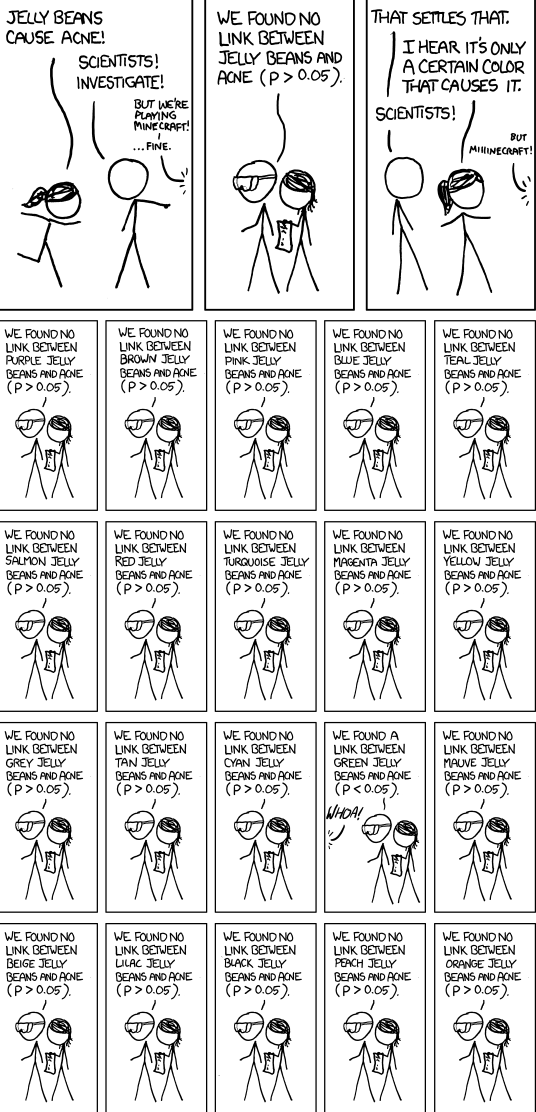
\includegraphics[height=0.97\textheight]{l3/significant_upper}}
			\end{center}
		\end{column}
		\begin{column}{0.4\textwidth}
			\href{https://www.xkcd.com/882/}{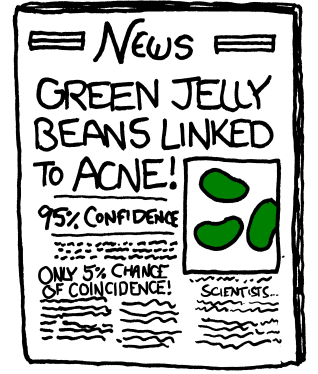
\includegraphics[width=0.5\textwidth]{l3/significant_news}}
		\end{column}
	\end{columns}
\end{frame}

\end{document}
